\documentclass[11pt]{article}

\usepackage{times}
\usepackage{epsf}
\usepackage{epsfig}
\usepackage{amsmath, alltt, amssymb, xspace}
\usepackage{wrapfig}
\usepackage{fancyhdr}
\usepackage{url}
\usepackage{verbatim}
\usepackage{fancyvrb}

\usepackage{subfigure}
\usepackage{cite}
%\usepackage{cases}
%\usepackage{ltexpprt}
%\usepackage{verbatim}

%\topmargin      -0.70in  % distance to headers
%\headheight     0.2in   % height of header box
%\headsep        0.4in   % distance to top line
%\footskip       0.3in   % distance from bottom line

% Horizontal alignment
\topmargin      -0.50in  % distance to headers
\oddsidemargin  0.0in
\evensidemargin 0.0in
\textwidth      6.5in
\textheight     8.9in 


%\centerfigcaptionstrue

%\def\baselinestretch{0.95}


\newcommand\discuss[1]{\{\textbf{Discuss:} \textit{#1}\}}
%\newcommand\todo[1]{\vspace{0.1in}\{\textbf{Todo:} \textit{#1}\}\vspace{0.1in}}
\newtheorem{problem}{Problem}[section]
%\newtheorem{theorem}{Theorem}
%\newtheorem{fact}{Fact}
\newtheorem{define}{Definition}[section]
%\newtheorem{analysis}{Analysis}
\newcommand\vspacenoindent{\vspace{0.1in} \noindent}

%\newenvironment{proof}{\noindent {\bf Proof}.}{\hspace*{\fill}~\mbox{\rule[0pt]{1.3ex}{1.3ex}}}
%\newcommand\todo[1]{\vspace{0.1in}\{\textbf{Todo:} \textit{#1}\}\vspace{0.1in}}

%\newcommand\reducespace{\vspace{-0.1in}}
% reduce the space between lines
%\def\baselinestretch{0.95}

\newcommand{\fixmefn}[1]{ \footnote{\sf\ \ \fbox{FIXME} #1} }
\newcommand{\todo}[1]{
\vspace{0.1in}
\fbox{\parbox{6in}{TODO: #1}}
\vspace{0.1in}
}

\newcommand{\mybox}[1]{
\vspace{0.2in}
\noindent
\fbox{\parbox{6.5in}{#1}}
\vspace{0.1in}
}


\newcounter{question}
\setcounter{question}{1}

\newcommand{\myquestion} {{\vspace{0.1in} \noindent \bf Question \arabic{question}:} \addtocounter{question}{1} \,}

\newcommand{\myproblem} {{\noindent \bf Problem \arabic{question}:} \addtocounter{question}{1} \,}


\newcommand{\copyrightnoticeA}[1]{
\vspace{0.1in}
\fbox{\parbox{6in}{\small Copyright \copyright\ 2006 - 2014\ \ Wenliang Du, Syracuse University.\\ 
      The development of this document is partially funded by 
      the National Science Foundation's Course, Curriculum, and Laboratory 
      Improvement (CCLI) program under Award No. 0618680 and 0231122. 
      Permission is granted to copy, distribute and/or modify this document
      under the terms of the GNU Free Documentation License, Version 1.2
      or any later version published by the Free Software Foundation.
      A copy of the license can be found at http://www.gnu.org/licenses/fdl.html.}}
\vspace{0.1in}
}


\newcommand{\copyrightnotice}[1]{
\vspace{0.1in}
\fbox{\parbox{6in}{\small Copyright \copyright\ 2006 - 2014\ \ Wenliang Du, Syracuse University.\\
      The development of this document is/was funded by three grants from
      the US National Science Foundation: Awards No. 0231122 and 0618680 from
      TUES/CCLI and  Award No. 1017771 from Trustworthy Computing.
      This lab was imported into the Labtainer framework by the Naval Postgraduate 
      School, Center for Cybersecurity and Cyber Operations under National Science 
      Foundation Award No. 1438893.
      Permission is granted to copy, distribute and/or modify this document
      under the terms of the GNU Free Documentation License, Version 1.2
      or any later version published by the Free Software Foundation.
      A copy of the license can be found at http://www.gnu.org/licenses/fdl.html.}}
\vspace{0.1in}
}

\newcommand{\copyrightnoticeB}[1]{
\vspace{0.1in}
\fbox{\parbox{6in}{\small Copyright \copyright\ 2006 - 2014\ \ Wenliang Du, Syracuse University.\\
      The development of this document is/was funded by the following grants from
      the US National Science Foundation: No. 0231122, 0618680, and 1303306.
      Permission is granted to copy, distribute and/or modify this document
      under the terms of the GNU Free Documentation License, Version 1.2
      or any later version published by the Free Software Foundation.
      A copy of the license can be found at http://www.gnu.org/licenses/fdl.html.}}
\vspace{0.1in}
}


\newcommand{\nocopyrightnotice}[1]{
\vspace{0.1in}
\fbox{\parbox{6in}{\small  
      The development of this document is funded by 
      the National Science Foundation's Course, Curriculum, and Laboratory 
      Improvement (CCLI) program under Award No. 0618680 and 0231122. 
      Permission is granted to copy, distribute and/or modify this document.
      }}
\vspace{0.1in}
}

\newcommand{\idea}[1]{
\vspace{0.1in}
{\sf IDEA:\ \ \fbox{\parbox{5in}{#1}}}
\vspace{0.1in}
}

\newcommand{\questionblock}[1]{
\vspace{0.1in}
\fbox{\parbox{6in}{#1}}
\vspace{0.1in}
}


\newcommand{\minix}{{\tt Minix}\xspace}
\newcommand{\unix}{{\tt Unix}\xspace}
\newcommand{\linux}{{\tt Linux}\xspace}
\newcommand{\ubuntu}{{\tt Ubuntu}\xspace}
\newcommand{\selinux}{{\tt SELinux}\xspace}
\newcommand{\freebsd}{{\tt FreeBSD}\xspace}
\newcommand{\solaris}{{\tt Solaris}\xspace}
\newcommand{\windowsnt}{{\tt Windows NT}\xspace}
\newcommand{\setuid}{{\tt Set-UID}\xspace}
%\newcommand{\smx}{{\tt Smx}\xspace}
\newcommand{\smx}{{\tt Minix}\xspace}
\newcommand{\relay}{{\tt relay}\xspace}
\newcommand{\isys}{{\tt iSYS}\xspace}
\newcommand{\ilan}{{\tt iLAN}\xspace}
\newcommand{\iSYS}{{\tt iSYS}\xspace}
\newcommand{\iLAN}{{\tt iLAN}\xspace}
\newcommand{\iLANs}{{\tt iLAN}s\xspace}
\newcommand{\bochs}{{\tt Bochs}\xspace}

\newcommand\FF{{\mathcal{F}}}

\newcommand{\argmax}[1]{
\begin{minipage}[t]{1.25cm}\parskip-1ex\begin{center}
argmax
#1
\end{center}\end{minipage}
\;
}

\newcommand{\bm}{\boldmath}
\newcommand  {\bx}    {\mbox{\boldmath $x$}}
\newcommand  {\by}    {\mbox{\boldmath $y$}}
\newcommand  {\br}    {\mbox{\boldmath $r$}}


%\pagestyle{fancyplain}
%\lhead[\thepage]{\thesection}      % Note the different brackets!
%\rhead[\thesection]{SEED Laboratories}
%\lfoot[\fancyplain{}{}]{Syracuse University} 
%\cfoot[\fancyplain{}{}]{\thepage} 

\newcommand{\tstamp}{\today}   
%\lhead[\fancyplain{}{\thepage}]         {\fancyplain{}{\rightmark}}
%\chead[\fancyplain{}{}]                 {\fancyplain{}{}}
%\rhead[\fancyplain{}{\rightmark}]       {\fancyplain{}{\thepage}}
%\lfoot[\fancyplain{}{}]                 {\fancyplain{\tstamp}{\tstamp}}
%\cfoot[\fancyplain{\thepage}{}]         {\fancyplain{\thepage}{}}
%\rfoot[\fancyplain{\tstamp} {\tstamp}]  {\fancyplain{}{}}

\pagestyle{fancy}
%\lhead{\bfseries Computer Security Course Project}
\lhead{\bfseries SEED Labs}
\chead{}
\rhead{\small \thepage}
\lfoot{}
\cfoot{}
\rfoot{}

\usepackage{listings}
\usepackage{color}

\definecolor{dkgreen}{rgb}{0,0.6,0}
\definecolor{gray}{rgb}{0.5,0.5,0.5}
\definecolor{mauve}{rgb}{0.58,0,0.82}

\lstset{frame=tb,
  language=C,
  aboveskip=3mm,
  belowskip=3mm,
  showstringspaces=false,
  columns=flexible,
  basicstyle={\small\ttfamily},
  numbers=none,
  numberstyle=\tiny\color{gray},
  keywordstyle=\color{blue},
  commentstyle=\color{dkgreen},
  stringstyle=\color{mauve},
  breaklines=true,
  breakatwhitespace=true,
  tabsize=3
}



\begin{document}

\begin{center}
{\LARGE The OSSEC Host Intrusion Detection System}
\vspace{0.1in}\\
\end{center}


\section{Overview}
This exercise provides hands-on experience with the OSSEC
host-based intrusion detection system (IDS).  This IDS is commonly used and serves as the core of commercial IDS products
\footnote{https://wazuh.com/}.  Like most IDS products, it applies a set of rules to identify attacks on computers.
And as with many host-based IDS systems, OSSEC relies to a large extent on 
logs messages captured by the underlying operating system.

The lab includes the following objectives:
\begin{itemize}
\item Configure OSSEC agents for client computers, i.e., those whose activity will be monitored by the OSSEC server.
\item Generate log-based events and observe resulting alerts generated by OSSEC.
\item Observe the effects of ``active responses'' to system events, e.g., disabling traffic from an offending source.
\item Configure a client agent to alert on changes to the ports that the computer is listening to.
\item Define a rule to alert on web server access to a particular URL.
\item Explore limitations and complications associated rule-based IDS.
\item Consider \textbf{system} security attack surface trade-offs related to introducing 5MB of privileged code, some of which 
consumes whatever an attacker feeds your computers.
\end{itemize}

\subsection{Background}
This lab assumes the student has some introduction to IDS systems and
some familiarity with Unix logging.

\section{Lab Environment}
This lab runs in the Labtainer framework,
available at http://nps.edu/web/c3o/labtainers.
That site includes links to a pre-built virtual machine
that has Labtainers installed, however Labtainers can
be run on any Linux host that supports Docker containers.

From your labtainer-student directory start the lab using:
\begin{verbatim}
    labtainer ossec
\end{verbatim}
A link to this lab manual will be displayed.

\section{Lab topology}
In addition to an OSSEC server, this lab includes a workstation and a web server.

\begin{figure}[H]
\begin{center}
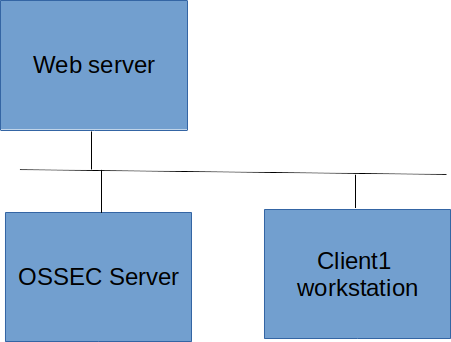
\includegraphics [width=0.8\linewidth]{ossec.png}
\end{center}
\caption{OSSEC Lab Topology}
\label{fig:topology}
\end{figure}

\section{OSSEC Operation}
Details on OSSEC can be found at \url{https://www.ossec.net/docs/index.html}.
The OSSEC server receives log entries from monitored computers via OSSEC agents that run on each monitored computer.  
A computer will not be monitored unless it has an agent installed and configured to communicate with the OSSEC server.
This communication requires:
\begin{itemize}
\item The client agent is registered on the OSSEC server and a cryptographic key is generated for the client.  Both
of these steps occur using the {\tt manage\_agents} command on the server.
\item The key is imported into the agent on the client, using the {\tt manage\_agents} command on the client.
\item The IP address of the server is defined in the client {\tt /var/ossec/etc/ossec.conf} file.
\item The {\tt ossec} service on the client and the server are each restarted.
\end{itemize}
Once those steps are complete, the server will begin to monitor the client based on log entries sent from the client
to the server.  The set of client logs to be monitored are defined in the {\tt ossec.conf} file on the client.
That file has a broad initial set of log files defined, though some of the log names may require modification as we
will see in this lab.

What the server does with received log messages is primarily defined in a set of \textit{rules} located in the 
server {\tt /var/ossec/rules} 
directory.  Server actions include generating alerts and causing active responses, e.g., directing a client to temporarily disable
network traffic from an offending source.  

Log messages are parsed and categorized based on \textit{decoding} rules defined in 
\begin{verbatim}
   /var/ossec/etc/decoder.xml
\end{verbatim}
\noindent OSSEC includes decoders for most common log formats.  The decoders assign identifiers to different types of log messages,
and these identifiers may then be named in rules.  For example, a decoder may assign selected messages generated by a web
server as being of type {\tt web-accesslog}.  A rule might then define an alert to be generated if it finds a message of 
type {\tt web-accesslog} to contain a character string indicative of an SQL injection attack. 

\section{Tasks}

\subsection{Configure OSSEC to monitor the client1 workstation}
The configuration files for each agent in the lab have been preconfigured to identify the server IP address.  So you only need
get keys into each agent to get them talking with the server.
Most OSSEC operations require use of sudo, so you might as well just "sudo su".
\begin{itemize}
\item On the server, run the {\tt /var/ossec/bin/manage\_agents} command to define an agent for the {\tt client1} computer and
to export a key for that client. (Just run the command, you'll figure it out.)
\item Copy the key that was generated on the server.
\item On the {\tt client1} computer, run the {\tt manage\_agents} command and import the key by pasting it when prompted.
\item Use {\tt systemctl restart ossec} on the client and the server.  
\end{itemize}

\subsection{Cause and observe alerts}
Out of the box, OSSEC monitors many different security relevant events, some of which get reported as \textit{alerts} in the
{\tt /var/ossec/logs/alerts/alerts.log} file in the server.  You'll be looking at that file a bit, so tail it in a new terminal:
\begin{itemize}
\item At the Labtainers terminal (labtainer-student), create a new terminal for the OSS computer:
\begin{verbatim}
    moreterm.py ossec ossec
\end{verbatim}
\item On the new terminal:
\begin{verbatim}
   sudo su
   tail -f /var/ossec/logs/alerts/alert.log
\end{verbatim}
\end{itemize}
Once you are monitoring alerts, create one.  Go to the client1 computer, which may still be in a sudo shell, i.e., with
the root {\tt \#} prompt.  Type {\tt exit} at that prompt, or {\tt sudo su} if not yet in a sudo shell. 
Switch back and forth from a sudo su shell.  Note the alerts in
the OSSEC alerts.log.  Those of you with Unix experience may recognize the alerts as being little more than system log 
messages, which they are.  

\subsection{Add the Web server and test log monitoring}
Use the {\tt manage\_agents} command on the server to add the web server agent.  Then use the {\tt manage\_agent} command
on the web server to import the generated key.\footnote{Note the lack of an \textit{s} on the end of this command on the
web server.  Command syntax varies between the Ubuntu configuration of OSS (on the client) and the CentOS configuration
on the web server.}  Restart the ossec service on the OSSEC server and on the web server, noting that the service name
on the web server is {\tt ossec-hids}.

You should have seen alerts in the alert log for each of these actions.  Now go to the client1 computer and ssh to the web server, 
providing a bogus password.  Note the alerts.  Again, these are triggered by standard Unix log messages, in this case generated
by the SSH daemon.

\subsection{Active responses}
Repeat your failed attempt to ssh from client1 to the web server.  Use ctl-C to break out the first failed password
attempt to speed things up (you are looking to run the ssh command multiple times).  
And keep repeating it until the ssh command just hangs and you see an alert such as:
\begin{verbatim}
** Alert 1619194381.6291: mail  - syslog,sshd,authentication_failures,
2021 Apr 23 16:13:01 (webserver) 172.0.0.4->/var/log/secure
Rule: 5720 (level 10) -> 'Multiple SSHD authentication failures.'
Src IP: 172.0.0.3
\end{verbatim}
\noindent The rule defining this alert assigns its importance as ``level 10'', 
and any level over 6 will trigger an active response.
You can see the active response definitions within the {\tt ossec.conf} file on the server.  The response is to alter the
iptables on the web server to block all traffic from client1.  You can observe this using {\tt iptables -L} on the web server,
assuming you are quick enough\footnote{iptables is a Linux function for filtering network traffic.  See the \textit{iptables2} 
lab and/or user ``man iptables'' to learn more about their use}.
The network blocking is set for 10 minutes by default, but we've changed that to 1 minute for this lab.  

\subsection{Monitor chages to command output}
So far we've looked at OSSEC monitoring of log file entries.  The IDS also lets you monitor the output of defined commands.
In this section, you will configure OSSEC to generate alerts if there are any changes to the network ports listened to by 
the web server.  The first step is to tell OSSEC on the web server about the command to monitor.  In this example, you wll 
monitor output of the {\tt netstat} command.  Enter this command on the web server:
\begin{verbatim}
    netstat -tan |grep LISTEN|grep -v 127.0.0.1
\end{verbatim}
\noindent The output shows which network ports are currently being listened to by the web server.  Your goal is to generate 
alerts when that output changes.  Edit the web server {\tt ossec.conf} file.  Note the different {\tt localfile} definitions.
Add a new {\tt localfile} entry at the end of the file, just above the last line.
\begin{verbatim}
    <localfile>
        <log_format>full_command</log_format>
        <command>netstat -tan |grep LISTEN|grep -v 127.0.0.1</command>
        <frequency>5</frequency>
    </localfile>
\end{verbatim}
\noindent  The {\tt log\_format} entry tells OSSEC you are defining a command that it is to periodically run.
The {\tt command} entry is the command you want it to run.  And the {\tt frequency} is how often, in seconds, that
you want to run the command.  After you restart the {\tt ossec-hids} service, OSSEC will start to periodically run
that command and send the output to the server.

Now, on the server, we need a rule to monitor that output.  There already is such a rule, which you can see in the
file at
\begin{verbatim}
/var/ossec/rules/ossec_rules.xml
\end{verbatim}

\noindent In that file, find rule 533, which is reproduced below.  
The rule format definitions can be found in the OSSEC web pages.  
\begin{verbatim}
  <rule id="533" level="7">
    <if_sid>530</if_sid>
    <pcre2>ossec: output: 'netstat -tan</pcre2>
    <check_diff />
    <description>Listened ports status (netstat) changed 
      (new port opened or closed).</description>
  </rule>

\end{verbatim}
\noindent This rule can be read as follows:  The id is an arbitrary number that identifies the rule.
The level is 7, which is high enough to generate an alert.  Rule classifications
are characterized at: \url{https://www.ossec.net/docs/docs/manual/rules-decoders/rule-levels.html}.

The {\tt if\_sid} entry reflects the OSSEC rule chaining strategy.  It says to consider this rule only if the event
already matched rule id 530, which is a rule that identifies output from monitored commands.
The {\tt pcre2} entry identifies which command output to evaluate, in this case, output from the netstat command defined
to run on the web server\footnote{pcre2 is a ``regular expression'' syntax.  This simple example just does a string match.
Use ``man pcre'' to learn more, and checkout regexone.com for a tutorial.}.  The {\tt check\_diff} entry tells OSSEC to generate alerts when the monitored messages change.

Close the file and restart the ossec service.  Then go to the web server and use the {\tt netcat} command to listen to some
arbitrary port, e.g.,
\begin{verbatim}
  nc -l 22345
\end{verbatim}

\noindent You should see a corresponding alert.   Then stop netcat using ctrl-c.  Note another alert, this time because the 
port was not longer being listened to.  Recall the frequency of our command output generation is every 5 seconds.  In a real 
deployment, you may wish to reduce the frequency so that the web server service can be updated and restarted without 
generating alerts.  On the  other hand, the lower the frequency, the more time rouge software has to listen to a port
without being detected.

\subsection{Monitor web resource access}
In this section, we'll create rules to monitor access to a specific web resource based on web log entries.  
The first step is to make sure our web logs are forwarded to the server.  

\subsubsection{Log locations}
Recall that log locations are defined
in the client's {\tt ossec.conf} file.  Open that file on the web server and find the entry for the web server,
which is apache. You will see two entries, one for the access log and one for the error log.  Neither match our
installation, which puts the logs in {\tt /var/log/httpd}.  Alter the 2 entries to reflect the log locations.
Then restart the {\tt ossec-hids} service.

You can confirm the agent is processing the expected logs by viewing the {\tt /var/ossec/logs/ossec.log} file.

\subsubsection{Rules testing}
OSSEC provides a tool to help create and test new rules, and we'll use this tool to help understand the structure
of the rules chains.  At the client1 workstation, issue the following web request from the command line\footnote{There
are several ways of making web requests, including curl, wget and browsers.  For most of this lab, please use curl.
You'll see why toward the end.}:
\begin{verbatim}
    curl 172.0.0.4
\end{verbatim}
\noindent At the web server, tail the access.log:
\begin{verbatim}
   tail -f /var/log/httpd/access.log
\end{verbatim}
\noindent At the OSSEC server start the {\tt ossec-logtest} program in verbose mode:
\begin{verbatim}
    /var/ossec/bin/ossec-logtest -v
\end{verbatim}
\noindent  This program will consume a log entry provided as standard input, and it will display its processing
steps and any alerts that would have been generated had the lab entry been real.  Copy the log entry from the web server's
access\_log and paste it into the server window where the logtest program is running.  Observe the output.

The first phase simply repeats the log entry.   The second phase reflects the results of decoding per the {\tt /var/ossec/etc/decocder.xml} file.  In this example, we
see the decoder has decoded this as a {\tt web-accesslog}, and it identifies a set of values defined for that log type,
including the success of the {\tt GET} command, which is 200 (successful).  The decoder assigns this decoding a
\textit{type} of {\tt web-log}, (unfortunately not reflected in the tools output.)   Phase 3 is the rules processing.

OSSEC rules processing for this example can be summarized 
as:  Start at the lowest numbered rule and find the first match. The ``rule 4''
in this example was found in the {\tt rules\_config.xml} file.  It then looks at rules having a category of 
{\tt web-log}, which includes rules defined in the {\tt web\_rules.xml} file, where it finds a match with rule ID 
31100.  It then searches for rules that are a ``child'' of rule 31100, i.e., those with an {\tt if\_sid} of 31100.
Again, it searches in order until it finds a match.  In this case the match is rule ID 31108, which represents itself
as ``Ignored URLs (simple queries)".  It then looks for a child of 31108 that matches the log entry.  We see it
tried rule 31103 and rule 31509, but did not find a match and thus halted with rule 31108 as the best match.
Since the rule has a level of 0, it is ignored and no alert is generated.

For our example purposes, that rule chain is fine because we don't care if that particular web page is accessed.  Our focus will
be on access to the {\tt 172.0.0.4/plan.html} page, (those of you who've performed the snort lab will recognize
these web pages).   Go back to the client workstation and use curl to retrieve the plan.html page.  Look at the 
web server log entry and consider how we can identify log entries reflecting access to the plan.html page.  
Obviously we can just look for that string.  So we'll create a new rule that looks for that string.

In order for our new rule to even be considered, it will have to be a child of rule 31108.  Though we may want to 
make the rule a child of 31100, we cannot because the OSSEC rules algorithm will always match the 31108 first. 
(OSSEC prescribes that you not
modify the existing OSSEC rules and follow the convention of putting new rules in the {\tt local\_rules.xml} file
with rule ID $>$ 100000).  Note this is a non-trivial constraint because rules are searched in order of rule ID.

Open the {\tt local\_rules.xml} file and add this rule:
\begin{verbatim}
  <rule id="140234" level="7">
    <if_sid>31108</if_sid>
    <url_pcre2>plan.html</url_pcre2>
    <description>Accessed the business plan.</description>
  </rule>

\end{verbatim}
Then re-run the {\tt ossec-logtest} (use ctlr-c to break out of a previous use of the program and then start the program
again.)

Once you've tested the rule and see that it works, restart the ossec service on the server and issue the curl request from 
the workstation again to confirm the alert appears in the alerts.log.

\subsubsection{Event coverage}
The new rule generates an alert when the plan.html resource is successfully accessed.  But does it always?
Alter your query to: {\tt 172.0.0.4/plan.html?}.  Do you seen an alert?  The question mark causes the rule parsing
to no long consider this log entry a simple query.  Run the log entry in the logtest program and view the processing.
Note the selected rule is 31100, which we've seen before.  To handle non-simple queries, we'd like a rule that is a
child of 31100.  OSSEC lets us make a rule that is a child to multiple other rules by including a comma-separated list
of IDs in the {\tt if\_sid} field.   Make that change to the new rule and test it.

\subsubsection{Failed attempts}
What about when someone tries
and fails to access the plan?  In other words, could we alert if it appears that someone is using brute force to try
to find the business plan?  At the client, try to retrieve this resource: 172.0.0.4/plan9.html.  Notice how no alert is
generated.  Go back to the logtest and view the processing of the new access log entry.

Create a new rule to generate an alert that reports the following when a failed attempt is made to access any 
resources with the string \textit{plan} in the URL.
\begin{verbatim}
    Attempt to access the business plan.
\end{verbatim}


\noindent To complete this lab, you must test your new rule along with the previous rule and demonstrate the following
by using curl at the client1:
\begin{itemize}
\item A query for {\tt plan.html} or {\tt plan.html?}generates the ``Accessed the business plan'' alert.
\item A query for {\tt plan9.html} generates the ``Attempt to access the business plan'' alert.
\item A query for {\tt about.html} does not generate any alert.
\end{itemize}

\subsection{Completeness (i.e., rat holes)}
Now that we have our web content rules in place, try one more experiment.  Instead of using {\tt curl},
use {\tt wget} on client1 to retrieve the resources in the list of queries above, and observe the alerts.  What is missing?
Use the logtest program to observe the rules processing on the log entry that failed to create the anticipated 
alert.  You need not correct the problem for this lab.  But do make note of this property of rules-based bolt-on
security mechanisms:  \textbf{You never know when you are done}.   This is often true when trying to protect
systems using IDS, anti-virus,
and rules-based ``mandatory access controls''.  

\subsection{Effects on system security}
On the client1 workstation, go to the /var/ossec/bin directory and view the directory content.  Use ps to see which 
ossec program run as root:
\begin{verbatim}
   ps aux | grep ossec
\end{verbatim} Note the
The {\tt ossec-logcollector} program is 167KB, without libraries, which can be seen using the ldd program:
\begin{verbatim}
    ldd ossec-logcollector
\end{verbatim}
Then go to the server computer and view its binaries and note which ones run as root.

While OSSEC does separate some processing to the non-root {\tt ossec} user, much processing is still performed by root,
and this includes collection of logs whose content may be determined by arbitrary external entities.

Any system contemplating use of an IDS should weigh the trade-offs associated with introducing large amounts of
privileged code into their systems.   

\subsubsection{Abuse of active responses}
Another system security consideration is the potential for abuse of active responses.  For example, how might an attacker
cause denial of service, preventing client1 from accessing the web server, just by causing some non-privileged program to
run on client1?  Or consider the case of an attacker having non-privileged access to client1 who would like ten minutes
of unobserved interaction with client1?  If client1 were the source of numerous failed ssh attempts to the OSSEC server itself,
what would be the result?

\section{Submission}
After finishing the lab, go to the terminal on your Linux system that was used to start the lab and type:
\begin{verbatim}
    stoplab 
\end{verbatim}
When you stop the lab, the system will display a path to the zipped lab results on your Linux system.  Provide that file to 
your instructor, e.g., via the Sakai site.

\copyrightnotice

\end{document}
